\documentclass[output=paper,colorlinks,citecolor=brown, language=chinese]{langscibook}
\author{Na Song\orcid{}\affiliation{INALCO-CRLAO}}


\title{The apprehensive function of a final enclitic particle in Baoding (Sinitic)}
\abstract{This paper aims to examine the apprehensive function of a final enclitic particle \textit{=lɛ.ia} in the Baoding dialect, a Mandarin dialect spoken in Northern China (Sinitic). This particle is restricted to future situations and its main pragmatic function is to require the addressee's involvement in order to avoid a potential undesirable situation. It mainly but not exclusively appears in independent clauses and originally has a temporal function. In this paper, we examine the semantic and syntactic constraints on \textit{=lɛ.ia}, its various functions, and we have a detailed look at the predicates that it co-occurs with. We argue that the apprehensive function of \textit{=lɛ.ia} is a semantic extension of its temporal function as an imminent future marker. We also investigate the possible source of the enclitic particle: \textit{=lɛ.ia} synchronically functions as a single unit but can be traced to two final enclitic particles: the enclitic \textit{=lɛ} which marks change of state, and the enclitic particle \textit{=ia} marking imminent future. These data on the Baoding dialect not only fill a gap in providing detailed data on apprehensional morphology in a broad sense from a Sinitic language, but also point to subtle semantic variations and restrictions in the grammatical expression of undesirability, and to the strong pragmatic expectation on the addressee.}


% \newcommand{\textit{=lɛ.ia}}{\textit{=lɛ.ia} }



%\let\eachwordone=\itshape

\IfFileExists{../localcommands.tex}{
   \addbibresource{../localbibliography.bib}
   \usepackage{tabularx,multicol}
\usepackage{url}
\urlstyle{same}

\usepackage{langsci-optional}
\usepackage{langsci-lgr}
\usepackage{langsci-gb4e}

\babelprovide[import]{hebrew}

\usepackage{paralist} %%may not be needed, currently used in questionnaire


%Siena added packages for introduction; not sure they are needed
\usepackage[normalem]{ulem}
\useunder{\uline}{\ul}{}

%from Treis:
\usepackage{listings}
\lstset{basicstyle=\ttfamily,tabsize=2,breaklines=true}

%%from Francez
% % % \usepackage{cjhebrew}
%\usepackage{tipa}  Also included by D&A, need to check with LSP whether to change it to language science tipa
\usepackage{leipzig}
%%from Dabkowski&AnderBois:

\usepackage[shortlabels]{enumitem} 
\usepackage{centernot}
\usepackage{arydshln}
\usepackage{newunicodechar}
\usepackage{csquotes}
%\let\sups\relax \usepackage{tipa} commented out on 7/3/25 Martina
% \usepackage[all]{nowidow}
\usepackage{listings} \lstset{basicstyle=\ttfamily}
\usepackage{multirow}
\usepackage{rotating}
\usepackage{pdflscape}
\usepackage{xspace}
%\usepackage{tabularx}
%\usepackage{multicol}
\usepackage{supertabular}
\usepackage{hhline}
\usepackage{bbding} %this package is for the checkmarks in Table 6 in Browne et al.

%\usepackage{qtree}
%\usepackage{tree-dvips}

\usepackage{array}
\usetikzlibrary{calc,tikzmark,matrix}
\usepgflibrary{shadings}
\usepackage{pifont}
%from Fedotov:

\usepackage{langsci-textipa}
%\usepackage{multirow}


%\usepackage{xeCJK}

%%%%%%%%%%%%%%%%%%%%%%%%%%%%%%%%%%%%%%%%%%%%%%%%%%%%
%%% EXAMPLES %%%%%%%%%%%%%%%%%%%%%%%%%%%%%%%%%%%%%%%
%%%%%%%%%%%%%%%%%%%%%%%%%%%%%%%%%%%%%%%%%%%%%%%%%%%% 

% if you want the source line of examples to be in
% italics, uncomment the following line
\renewcommand{\exfont}{\itshape}
% to add additional information to the right of
% examples, uncomment the following line

%\usepackage{langsci/styles/jambox}


%%% FOOTNOTE EXAMPLE NUMBERING
% \makeatletter
% \patchcmd{\@footnotetext}{\setcounter{fnx}{0}}{\renewcommand{\thexnumi}{\roman{xnumi}}}{}{}
% \apptocmd{\@footnotetext}{
%     \@noftnotetrue
%     \renewcommand{\thexnumi}{\arabic{xnumi}}%
% }{}{}
%
% \makeatother
\usepackage[linguistics,edges]{forest}
\usepackage{hyphenat}
\usepackage{langsci-branding}

   \makeatletter
\let\thetitle\@title
\let\theauthor\@author
\makeatother

\newcommand{\togglepaper}[1][0]{
   \bibliography{../localbibliography}
   \papernote{\scriptsize\normalfont
     \theauthor.
     \titleTemp.
    To appear in:
    Martina Faller,  Marine Vuillermet \&  Eva Schultze-Berndt (eds.). Apprehensional Constructions in a cross-linguistic perspective. Berlin: Language Science Press. [preliminary page numbering]
   }
   \pagenumbering{roman}
   \setcounter{chapter}{#1}
   \addtocounter{chapter}{-1}
}

\newbool{bookcompile}
\booltrue{bookcompile}
\newcommand{\bookorchapter}[2]{\ifbool{bookcompile}{#1}{#2}}


\newfontfamily\FedotovBoldEmptySetFont{LibertinusSerif-Italic.otf}[AutoFakeBold=2.5]
\newcommand{\FedotovBoldEmpty}{{\FedotovBoldEmptySetFont\bfseries ∅}}

%From Dabkowski&AnderBois


\let\sc\scshape
\let\rm\rmfamily
%\let\it\itshape
\let\tt\ttfamily
\let\nr\normalfont

\newcommand{\wsc}[1]{\textls[80]{\scshape#1}}

\let\textai\textit
% \let\textlc\spacedlowsmallcaps
% \let\textac\spacedallcaps
\let\textlc\textsc
\let\textac\textsc


%%%%%%%%%%%%%%%%%%%%%%%%%%%%%%%%%%%%%%%%%%%%%%%%%%%%
%%% FLAG %%%%%%%%%%%%%%%%%%%%%%%%%%%%%%%%%%%%%%%%%%%
%%%%%%%%%%%%%%%%%%%%%%%%%%%%%%%%%%%%%%%%%%%%%%%%%%%%

% \newcommand{\scott}  [1]{\textcolor{violet}{#1}}
% \newcommand{\maks}   [1]{\textcolor{blue}{#1}}
% % \newcommand{\data}   [1]{\textcolor{teal}{#1}}
% \newcommand{\new}   [1]{#1}
% \newcommand{\newnew}   [1]{\textcolor{teal}{#1}}
% \newcommand{\rev}   [1]{\textcolor{magenta}{#1}}



%%%%%%%%%%%%%%%%%%%%%%%%%%%%%%%%%%%%%%%%%%%%%%%%%%%%
%%% TABLES %%%%%%%%%%%%%%%%%%%%%%%%%%%%%%%%%%%%%%%%%
%%%%%%%%%%%%%%%%%%%%%%%%%%%%%%%%%%%%%%%%%%%%%%%%%%%%

%\newcolumntype{Y}{>{\arraybackslash}p{25.3543464286pt}} % length of L

% \newcolumntype{K}{>{\arraybackslash}p{24.25pt}}
% \newcolumntype{V}{>{\arraybackslash}p{(\textwidth/9-24pt)/2}}
%
\let\ch\relax \newcommand{\ch}[2]{\multicolumn{#1}{c}{\sc#2}}
\let\sx\relax \newcommand{\sx}[2]{\multicolumn{#1}{l}{\emph{-#2}}} % suffix
\let\su\relax \newcommand{\su}{\sx{1}} % suffix unicolumnal
\let\sd\relax \newcommand{\sd}{\sx{2}} % suffix dicolumnal
\let\cx\relax \newcommand{\cx}[2]{\multicolumn{#1}{l}{\emph{=#2}}} % clitic
\let\cu\relax \newcommand{\cu}{\cx{1}} % clitic unicolumnal
\let\cd\relax \newcommand{\cd}{\cx{2}} % suffix dicolumnal
\let\gx\relax \newcommand{\gx}[2]{\multicolumn{#1}{l}{\sc #2}} % gloss
\let\gd\relax \newcommand{\gd}{\gx{2}} % gloss dicolumnal
\let\gr\relax \newcommand{\gr}[1]{\multicolumn{2}{c}{\multirow{2}{*}{\textcolor{gray}{\sc#1}}}}
\let\db\relax \newcommand{\db}[1]{\multicolumn{2}{c}{\multirow{2}{*}{\sc#1}}}



%%%%%%%%%%%%%%%%%%%%%%%%%%%%%%%%%%%%%%%%%%%%%%%%%%%%
%%% EXAMPLES %%%%%%%%%%%%%%%%%%%%%%%%%%%%%%%%%%%%%%%
%%%%%%%%%%%%%%%%%%%%%%%%%%%%%%%%%%%%%%%%%%%%%%%%%%%%

%%% AFFIX BOUNDARY %%%%%%
% \DeclareRobustCommand{\longmn}{\textminus}
% \DeclareRobustCommand{\mn}{-}

%%% CLITIC BOUNDARY %%%%%%
% \DeclareRobustCommand{\longeq}{=}
% \makeatletter\DeclareRobustCommand{\eq}{%
%     \settowidth{\@tempdima}{-}% width of a hyphen
%     \resizebox{\@tempdima}{\height}{=}%
% }\makeatother

%%% FUZZY CLITIC %%%%%%
% \DeclareRobustCommand{\longfc}{%
%     $\overset{\text{\smash{}}}{\text{$\approx$}}$%
% }
% \makeatletter\DeclareRobustCommand{\fc}{%
%     \settowidth{\@tempdima}{-}% width of a hyphen
%     \resizebox{\@tempdima}{\height}{%
%         $\overset{\text{\smash{}}}{\text{$\approx$}}$%
%     }%
% }\makeatother

%%% REDUPLICATION %%%%%%%
% \DeclareRobustCommand{\longtl}{$\sim$}
% \makeatletter\DeclareRobustCommand{\tl}{%
%     \settowidth{\@tempdima}{-}% width of a hyphen
%     \resizebox{\@tempdima}{\height}{$\sim$}%
% }\makeatother

% \newcommand{\mn}          {\textminus}
\newcommand{\src}    [1]  {\jambox[0pt]{\rm(#1)}}
% \newcommand{\ai}     [2]  {\emph{#1} `\textsc{#2}#3'\xspace}
\newcommand{\ai}     [2]  {\emph{#1} `\textsc{#2}'\xspace}
\newcommand{\sane}   [1][]{\ai{=sa'ne}{appr}{#1}}
\newcommand{\srcn}   [1][]{\ai{kûintsû}{srcn}{#1}}
% \newcommand{\mbekane}[1][]{\ai{\eq mbe kañe}{neg.adv aux.inf}{#1}}

% \let\sc\relax \newcommand{\sc}{\normalfont\scshape}
% \let\rm\relax \newcommand{\rm}{\normalfont\rmfamily}
% \let\it\relax \newcommand{\it}{\normalfont\itfamily}

\newcommand{\lb}{{\rm[}}
\newcommand{\rb}{{\rm]}}

\newcommand{\bad}{\makebox[0pt][r]{*\,}}
\newcommand{\infel}{\makebox[0pt][r]{\#\,}}


% \newcommand{\lsqz}[1]{#1}
% \newcommand{\lsqz}[1]{\makebox[0pt][l]{#1}}

% \newcommand{\lsqu}[1]{\makebox[0pt][l]{#1}}
% \newcommand{\rsqu}[1]{\makebox[0pt][r]{#1}}
% \newcommand{\astr}{\makebox[0pt][r]{{\nr*}}}
% \newcommand{\hash}{\makebox[0pt][r]{{\nr\#}}}
% \newcommand{\qstn}{\makebox[0pt][r]{{\nr?}}}
% \newcommand{\bad}{\makebox[0pt][r]{*}}
% \newcommand{\unhappy}{\makebox[0pt][r]{\#}}


%%%%%%%%%%%%%%%%%%%%%%%%%%%%%%%%%%%%%%%%%%%%%%%%%%%%
%%% UNICODE CHARACTERS  %%%%%%%%%%%%%%%%%%%%%%%%%%%%
%%%%%%%%%%%%%%%%%%%%%%%%%%%%%%%%%%%%%%%%%%%%%%%%%%%%

\newunicodechar{⟨}{⟨}
\newunicodechar{⟩}{⟩}

\newcommand{\infix}{⟨}
\newcommand{\outfix}{⟩}



%%%%%%%%%%%%%%%%%%%%%%%%%%%%%%%%%%%%%%%%%%%%%%%%%%%%
%%% IPA %%%%%%%%%%%%%%%%%%%%%%%%%%%%%%%%%%%%%%%%%%%%
%%%%%%%%%%%%%%%%%%%%%%%%%%%%%%%%%%%%%%%%%%%%%%%%%%%%

% \newcommand{\ipa}{\textipa}

\newcommand{\sub}{\textsubscript}
% \let\super\relax \newcommand{\super}{\textsuperscript}

\newcommand{\ts}{\texttslig}
% \let\dz\relax \newcommand{\dz}{\textdzlig}
\newcommand{\tS}{\textteshlig}
\newcommand{\dZ}{\textdyoghlig}
\newcommand{\cj}{\textctc}
\newcommand{\sj}{\textctc}
\newcommand{\zj}{\textctz}
\newcommand{\tcj}{\texttctclig}
\newcommand{\tsj}{\texttctclig}
\newcommand{\dzj}{\textdctzlig}
\newcommand{\gj}{\textbardotlessj}
% \let\nj\relax \newcommand{\nj}{\textltailn}
% \newcommand{\W}{\textturnmrleg}
\newcommand{\wl}{\textturnmrleg}
% \newcommand{\1}{\ipabar{\~\i}{.5ex}{1.1}{}{}}
\newcommand{\dotlessibar}{\ipabar{\i}{.5ex}{1.1}{}{}}
\newcommand{\darkl}{\textltilde}
% \newcommand{\n}{\textsubarch}
% \newcommand{\x}{\textovercross}
\newcommand{\lowered}{\textlowering}
\newcommand{\raised}{\textraising}
\newcommand{\retracted}{\textsubbar}
\newcommand{\unreleased}{\textcorner}
% \newcommand{\syllabic}{\s}
\newcommand{\implosivet}{\texthtt}
\newcommand{\implosived}{\texthtd}
\newcommand{\implosivep}{\texthtp}
\newcommand{\implosiveb}{\texthtb}
\newcommand{\implosivek}{\texthtk}
\newcommand{\implosiveg}{\texthtg}



%%%%%%%%%%%%%%%%%%%%%%%%%%%%%%%%%%%%%%%%%%%%%%%%%%%%
%%% OTHER %%%%%%%%%%%%%%%%%%%%%%%%%%%%%%
%%%%%%%%%%%%%%%%%%%%%%%%%%%%%%%%%%%%%%%%%%%%%%%%%%%%

\newcommand{\ie}{i.\,e.\xspace}
\newcommand{\Ie}{I.\,e.\xspace}
\newcommand{\eg}{e.\,g.\xspace}
\newcommand{\Eg}{E.\,g.\xspace} 




\newcommand{\francoissource}[1]{\hfill\textnormal{{\footnotesize #1} }}
\newcommand{\E}{Ɛ\kern-1.5pt\raisebox{1pt}{̏}\kern1.5pt}
\newcommand{\ù}{{ṵ}\kern-2pt{̀}\kern2pt}
\newcommand{\ȕ}{{ṵ}\kern-2pt{̏}\kern2pt}

\newcommand{\OO}{ɔ\kern-1pt\raisebox{-1pt}{̰}\kern1pt}
\newcommand{\Ǒ}{{{ɔ̌\kern-1pt\raisebox{-.5pt}{̰}\kern1pt}}}


\newcommand{\à}{{a̰}\kern-2pt{̀}\kern2pt}
\newcommand{\ilit}[1]{#1\il{#1}}

   %% hyphenation points for line breaks
%% Normally, automatic hyphenation in LaTeX is very good
%% If a word is mis-hyphenated, add it to this file
%%
%% add information to TeX file before \begin{document} with:
%% %% hyphenation points for line breaks
%% Normally, automatic hyphenation in LaTeX is very good
%% If a word is mis-hyphenated, add it to this file
%%
%% add information to TeX file before \begin{document} with:
%% %% hyphenation points for line breaks
%% Normally, automatic hyphenation in LaTeX is very good
%% If a word is mis-hyphenated, add it to this file
%%
%% add information to TeX file before \begin{document} with:
%% \include{localhyphenation}

\hyphenation{
par-a-digm
com-ple-men-ta-tion
anaph-o-ra
Dor-drecht
Cu-shi-tic
be-ne-dic-tive
pa-ra-digms
Ethi-o-pi-an
hoch-land-ost-ku-schi-ti-schen 
Duu-raa-me
Pa-ken-dorf
Lich-ten-berk
affri-ca-te
affri-ca-tes
com-ple-ments
Eng-lish
}




\hyphenation{
par-a-digm
com-ple-men-ta-tion
anaph-o-ra
Dor-drecht
Cu-shi-tic
be-ne-dic-tive
pa-ra-digms
Ethi-o-pi-an
hoch-land-ost-ku-schi-ti-schen 
Duu-raa-me
Pa-ken-dorf
Lich-ten-berk
affri-ca-te
affri-ca-tes
com-ple-ments
Eng-lish
}




\hyphenation{
par-a-digm
com-ple-men-ta-tion
anaph-o-ra
Dor-drecht
Cu-shi-tic
be-ne-dic-tive
pa-ra-digms
Ethi-o-pi-an
hoch-land-ost-ku-schi-ti-schen 
Duu-raa-me
Pa-ken-dorf
Lich-ten-berk
affri-ca-te
affri-ca-tes
com-ple-ments
Eng-lish
}



   \boolfalse{bookcompile}
   \togglepaper[23]%%chapternumber
}{}

\begin{document}
\maketitle

\section{Introduction}
%\label{sec:intro}

Languages may have different ways of encoding potential undesirable events which may be more or less grammaticalized. As a general characterization, apprehensive markers are semantically specialized markers that denote a potential event that is considered undesirable. They are also known as a modality that combines both epistemic and attitudinal components \citep[293]{lichtenberk1995}.

As a category, the apprehensive has not received a lot of attention cross-linguistically, apart from a handful of studies on Austronesian languages \citep{lichtenberk1995}, Amazonian languages \citep{vuillermet2018a} and Australian languages (\cite{Dixon2002}, \cite[255--296]{AngeloSchultze-Berndt2016}, \cite{Verstraete2005} among others).

Cross-linguistically, apprehensive marking may take the form of an independent word/particle as in To'aba'ita \citep{lichtenberk1995} or Northern Australian Kriol \citep{AngeloSchultze-Berndt2016}, or of an affix as in Yukulta \citep[247]{Keen1983} or in Ese Ejja \citep{vuillermet2018a}. In Sinitic languages, the apprehensive morpheme can be a modal adverb or a clausal linker as is described for Standard Mandarin (\sectref{subsec:apprmandarin}). In Baoding the apprehensive is primarily expressed by means of  a modal enclitic particle (\sectref{subsec:apprbaoding} and following sections).

An example of a morpheme in apprehensive function as defined above is \REF{ex:Song1}. As noted by \citet[102]{Merlan1983}, in Ngalakan, a northern non-Pama–Nyungan language in Australia, the evitative (apprehensive) prefix \textit{mele-} is used in an independent clause expressing some possible event which is deemed undesirable, rather than in a subordinate clause. 

\ea
\label{ex:Song1} 
\langinfo{Ngalakan}{Gunwinyguan/Ngalakan: Australia}{\cite[102]{Merlan1983}} \\
\gll Gu-wol-nowi \textbf{mele}-bolk. \\
\textsc{clf}-smoke-\textsc{3sg.poss} \textbf{\textsc{evit}}-get.out \\
\glt `The smoke might come out.'
\z

 \citet[168]{green1989} contrasts the apprehensional constructions in main vs.\ subordinate clauses in Marrithiyel (a language of the Daly River region of Australia's Northern Territory) by highlighting that in a main clause, the apprehensional marking expresses the speaker's view that the event is undesirable, while in subordinate clauses it expresses the subject's view.

\ea
\label{ex:Song2} 
\langinfo{Marrithiyel} {Western Daly, Australia}{\cite[80; 170]{green1989}} \\
\gll Gu-n-ning-pirr-\textbf{Ø-fang}. \\
\textsc{3S.r-}go-\textsc{1sg.O-nsg.nirr.S-}leave-\textsc{3pl-\textbf{appr}} \\
\glt `(I'm afraid) they might leave me.'
\z


\noindent In \REF{ex:Song2}, the apprehensive verbal suffix \textit{-fang} appears in a main clause. Leaving may not necessarily correspond to an undesirable situation, but the apprehensive markers actually encodes that, from the speaker's point of view, the event is undesirable. A similar situation is also found in Baoding (see \sectref{subsec:apprparticle} and \sectref{sec:semanticsleia}). \citet[202]{verstraete2006b} finds that in almost all his examples of Australian languages the apprehensional construction can be used in a main clause, most typically in warnings. 

Another topic which has recently drawn attention is the origin of apprehensional constructions. In Northern Australian Kriol, the temporal particle \textit{bambai} `later' coexists with a homophonous grammaticalized apprehensive particle, which displays a distinct syntactic  behaviour in addition to its specialized semantics.

\ea 
\label{ex:Song3} 
\langinfo{Kriol} {English-lexified creole language, Northern Australia} {\cite[269]{AngeloSchultze-Berndt2016}} \\
\ea \label{ex:Song3a}
\gll Ai show yu thad lilgel \textbf{bambai}, Denise, yu luk la im. \\
\textsc{1sg} show \textsc{2sg} \textsc{dem} girl \textbf{later} \textsc{name} \textsc{2sg} look \textsc{loc/all} \textsc{3sg} \\
\glt `I'll show you (=introduce you to) that girl later, Denise, you'll see her.' \\
\ex \label{ex:Song3b}
\gll Ai gan lad=i yu insaid. \textbf{Bambai} yu dagat mi. \\
\textsc{1sg} \textsc{can.neg} let=\textsc{tr} \textsc{2sg} inside \textbf{\textsc{appr}} \textsc{2sg} eat \textsc{1sg} \\
\glt `I won't let you in. You might eat me.'
\z
\z

 Concerning Sinitic languages, there are only few relevant studies, which concern adverbial apprehensional markers that could be grammaticalized from `fear' verbs in Standard Mandarin \citep{Gao2003}. This paper provides data from Baoding, a Mandarin dialect of the Sinitic group. 

\begin{figure}
    \caption{Location of Baoding, Hebei, China \citep[27]{song2020}}
    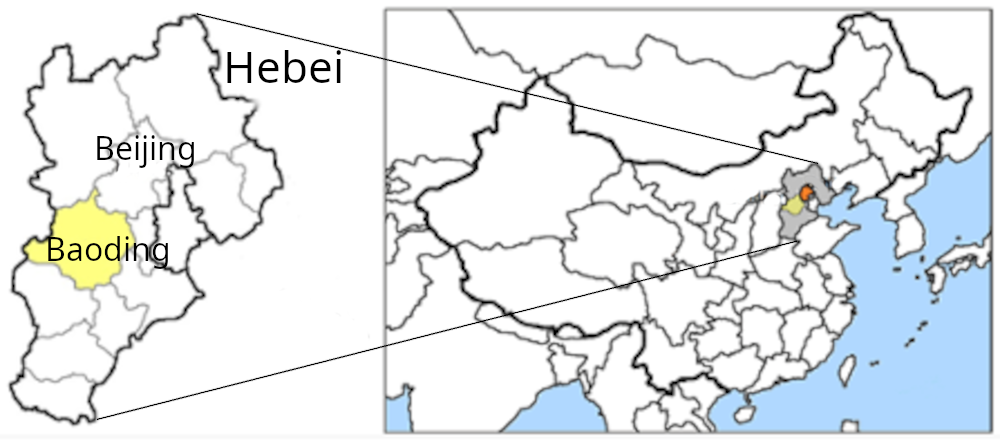
\includegraphics[width=\textwidth]{figures/location_mod.png}
    \label{fig:1}
\end{figure}

Baoding is located in Hebei province (China) and is about 140 km south of Beijing. According to The Language Atlas of China (Maps B 1-3, \cite{Liu2012}), the Baoding dialect belongs to the Jì-lŭ subgroup of Mandarin (a subgroup spoken in a large part of the Hebei province and in the western part of the Shandong province). Although the precise number of Baoding speakers is unknown, we can estimate that about the elder half of the population of the city  are likely to speak the Baoding dialect; due to the promotion of Standard Mandarin, younger speakers under 35 have lost their skills in the local language. Despite the geographical proximity of the Baoding dialect and the Beijing dialect, on which Standard Mandarin is based, the Baoding dialect possesses some syntactic features which are quite different from Standard Mandarin, notably in its Tense, Aspect, Modality, and Evidentiality (TAME) system. 

The data presented in this article are taken from the author's personal fieldwork data, gathered during a total of five months in a period extending from 2012 to 2017, which includes elicited sentences, in addition to approximately 40 hours of daily conversation. Our language consultants are around the age of 60 (two females and one male).

In this paper, I will show that besides the adverbial apprehensional markers grammaticalized from `fear' verbs described for Standard Mandarin (see \sectref{sec:apprsinitic}), Baoding may also express apprehension through a final enclitic particle in a main clause. This particle, \textit{=lɛ.ia}, has two main functions: a temporal function, when it encodes an imminent future event, and an apprehensive function with certain types of verbs (see \sectref{subsec:apprparticle}), which is related to speaker vs.\ addressee involvement: the particle is used to require the addressee's involvement in order to avoid a potential undesirable situation as illustrated in the following example:

\ea\label{ex:Song4} \textnormal{Baoding}\\
\gll Pã\textsuperscript{213} tɕiɛ̃\textsuperscript{213-21} tiɑ˞, tʰiɔ\textsuperscript{213-21}=\textbf{lɛ.ia.} \\
tie fasten a.little fall=\textsc{\textbf{appr}} \\
\glt `Tie it up a little bit, it's falling!' (Context: The speaker requires her husband to tie up the flour bag (25kg) at the back of his bicycle when she sees the bag is falling.)
\z

This paper is structured as follows: the current section has provided a general overview of the apprehensive as a cross-linguistic category. \sectref{sec:apprsinitic} presents the apprehensive morphemes in Standard Mandarin and a similar strategy in Baoding. After introducing the TAME system and the final enclitics in Baoding, \sectref{sec:leia} focuses on the apprehensive function of \textit{=lɛ.ia}, its distribution, and the predicates with which it co-occurs. \sectref{sec:semanticsleia} analyses the semantic contribution of \textit{=lɛ.ia}. \sectref{sec:leiaperson} discusses how \textit{=lɛ.ia}  interacts with person and with sentence type (polar questions). \sectref{sec:source} proposes a hypothesis on the source of \textit{=lɛ.ia} and tries to give an account of the semantic and pragmatic links between its temporal and apprehensive functions. \sectref{song-conclusion} concludes and gives some further perspectives on the motivation for this semantic change.


\section{Apprehensional constructions in Sinitic Languages}
\label{sec:apprsinitic}

\subsection{Apprehensive morphemes in Standard Mandarin}
\label{subsec:apprmandarin}

In Sinitic Languages, apprehensive morphemes have been described for Standard Mandarin by \citet{Gao2003}, with reference to \citegen{lichtenberk1995} study. She describes three morphemes  which could have an apprehensional use: \textit{pà}, \textit{kàn} and \textit{bié}, whose respective sources are a `fear' verb, a `see' verb, and a prohibitive marker. The following examples \REF{ex:Song5a} and \REF{ex:Song5b} illustrate the lexical and grammatical uses, respectively, of \textit{pà} in Standard Mandarin:

\ea \label{ex:Song5} 
\langinfo{Standard Mandarin} {Sinitic, Sino-Tibetan} {\cite{Gao2003}} \\
\ea \label{ex:Song5a} {\cn 老鼠怕猫。}\\
\gll Lǎoshǔ	\textbf{pà} māo. \\
mouse \textbf{fear} cat \\
\glt `A mouse fears cats.' \\
\ex \label{ex:Song5b} {\cn 老没见赵老师露面，怕是叫外国人请去演讲了。} \\
\gll Lǎo méi jiàn {Zhào lǎoshī} lòumiàn, \textbf{pà} shì jiào wàiguórén qĭng qù yǎnjiǎng le. \\
always \textsc{neg} see prof.Zhao show.up \textbf{\textsc{pot}} be \textsc{pass} foreigner invite go give.a.lecture \textsc{cos} \\
\glt `(I) have not seen Prof. Zhao put in an appearance. He might be away on an invitation by foreigners to give a lecture.' \\
\ex \label{ex:Song5c} {\cn 红云软软的说着，怕他不明白。}\\
\gll Hóngyún ruǎnruǎnde shuō, \textbf{pà} tā bù míngbai. \\
Hongyun gently speak \textsc{\textbf{appr}} \textsc{3sg} \textsc{neg} understand \\
\glt `Hongyun speaks gently, lest he does not understand.'
\z
\z

\noindent Example \REF{ex:Song5c} illustrates the apprehensional use of \textit{pà}: the morpheme has undergone a process of decategorialization \citep[104]{HopperTraugott1993} and it is on the way of the grammaticalization into a general potential modal adverb.

The prohibitive adverb \textit{bié} meaning `do not do something' as in \REF{ex:Song6a} can be also employed to mark the apprehensive as shown in \REF{ex:Song6b}:

\newpage
\ea \label{ex:Song6} 
\langinfo{Standard Mandarin} {Sinitic, Sino-Tibetan} {\cite{Gao2003}} \\
\ea \label{ex:Song6a} {\cn 别着急。}\\
\gll \textbf{Bié} zháojí. \\
\textbf{\textsc{neg$_{\mathrm{\textsc{proh}}}$}} worry \\
\glt `Don't worry.' \\
\ex \label{ex:Song6b} {\cn 看看去，别是一楼下水道又堵了。}\\
\gll Kànkan qu, \textbf{bié} shì yīlóu xiàshuĭdào yòu dǔ le.  \\
look.\textsc{red} go \textsc{\textbf{appr}} be first.floor sewer again block \textsc{cos} \\
\glt `Go and have a look. Maybe the sewer of the first floor got blocked up again.' [lit: `Let it not be the sewer of the first floor which got blocked up again.']
\z
\z

 The last morpheme is \textit{kàn}, which originally means `to see'. The source of this apprehensive marker is the complement-taking verb \textit{kán} `see'. Examples \REF{ex:Song7a} and \REF{ex:Song7b} illustrate, respectively, its verbal use and its apprehensive use in a threat.


\ea \label{ex:Song7} 
\langinfo{Standard Mandarin} {Sinitic, Sino-Tibetan} {\cite{Gao2003}} \\
\ea \label{ex:Song7a} {\cn 我看他拿了几本书走了。} \\
\gll Wǒ \textbf{kàn} tā ná le jĭ běn shū zǒu le. \\
\textsc{1sg} \textbf{see} \textsc{3sg} take \textsc{pfv} several \textsc{clf} book leave \textsc{cos} \\
\glt `I saw him take several books and leave.' \\
\ex \label{ex:Song7b} {\cn 再麻烦，看我带你到局里去!} \\
\gll Zài máfan, \textbf{kàn} wǒ dài nĭ dào jú li qu! \\
again bother \textsc{\textbf{appr}} \textsc{1sg} take \textsc{2sg} go.to police.station \textsc{loc} \textsc{go\&do} \\
\glt `If (you) bother (me) again, I will take you to the police station!'
[lit.: `You'll see that I will take you to the police station.']
\z
\z

 Similar apprehensive markers derived from `fear' verbs, `see' verbs and a prohibitive marker are also attested in Baoding, a non-standard variety of Mandarin spoken in Northern China.



\subsection{A standard Mandarin-like strategy of apprehensive morphemes in Baoding}
\label{subsec:apprbaoding}


Baoding has two strategies for expressing apprehension. Firstly, Baoding may use markers grammaticalized from complement-taking verbs such as `to fear', `to see' and from the prohibitive morpheme, similarly to Standard Mandarin, as illustrated in \REF{ex:Song8a}--\REF{ex:Song8b}.



\ea \label{ex:Song8} \textnormal{Baoding}\\
\ea \label{ex:Song8a}
\gll Tʰa\textsuperscript{45} \textbf{pʰa\textsuperscript{51}} tʰa\textsuperscript{45} pa\textsuperscript{51}. \\
\textsc{3sg} \textbf{fear} \textsc{3sg} father \\
\glt `She is afraid of her father.' \\
\ex \label{ex:Song8b}
\gll Uɤ\textsuperscript{213} te\textsuperscript{51} tso\textsuperscript{51} ti pɔ\textsuperscript{22} \textbf{pʰa\textsuperscript{51}} ni\textsuperscript{213} tʂʰʅ\textsuperscript{45-35}-tʂo ɕiæ̃\textsuperscript{22}. \\
\textsc{1sg} deliberately do \textsc{past} tasteless \textsc{\textbf{appr}} \textsc{2sg} eat-\textsc{sta} salty \\
\glt `I did (the meal) with less salt deliberately lest you find it too salty.' [lit.: `you eat it salty.'] \\
\ex \label{ex:Song8c}
\gll ɕiæ̃\textsuperscript{45} tɕʰi\textsuperscript{51-45} kɤ tiæ̃\textsuperscript{51}xua\textsuperscript{51}, \textbf{pʰa\textsuperscript{51}} tha\textsuperscript{45} pɛ\textsuperscript{22} pʰɔ\textsuperscript{213} i\textsuperscript{45-35} tʰɑ̃. \\
first make \textsc{clf} phone.call \textsc{\textbf{appr}} \textsc{3sg} in.vain run one trip \\
\glt `Give (him) a phone call first, lest he goes there in vain (lest he has a wasted journey).'
\z
\z

 As mentioned earlier, the verb \textit{pà} or \textit{kongpa} `fear' in Standard Mandarin is grammaticalizing into a general potential modal adverb and is not a dedicated apprehensional marker. By contrast, grammaticalized \textit{pʰa$^{51}$} in (\ref{ex:Song8b})--(\ref{ex:Song8c}), expresses both probability and undesirability, and functions as a dedicated apprehensional, namely a precautioning (`lest') clause.


The examples in \REF{ex:Song9} parallel the Standard Mandarin examples in \REF{ex:Song6}. In example \REF{ex:Song9b}, \textit{piɛ\textsuperscript{51}} is no longer a prohibitive adverb as in \REF{ex:Song9a}. Instead, it is used to express the speaker's wish or hope that an undesirable situation will not turn out to be true. In the same way, it concerns the speaker's fear that the undesirable event will take place. 


\ea \label{ex:Song9}  \textnormal{Baoding}\\
\ea \label{ex:Song9a}
\gll \textbf{Piɛ\textsuperscript{51}} lɔ\textsuperscript{213} nɔ\textsuperscript{22}iɑ˞\textsuperscript{213-21}=lɛ. \\
\textbf{\textsc{neg$_{\mathrm{\textsc{proh}}}$}} always stay.late.at.night=\textsc{cos} \\
\glt `Don't always stay late at night.' \\
\ex \label{ex:Song9b}
\gll Tsæ̃\textsuperscript{22}mɛ̃ mɑ̃\textsuperscript{22}xuɤ-lɛ pæ̃\textsuperscript{51}tʰiæ̃\textsuperscript{45} \textbf{piɛ\textsuperscript{51}} io\textsuperscript{51} pu\textsuperscript{45} tɕʰi\textsuperscript{51-45}=lo.  \\
\textsc{1incl} be.busy.with long.time \textsc{\textbf{appr}} again \textsc{neg} go=\textsc{irr} \\
\glt `We were busy with it for a long time. (I hope that it) won't be cancelled again.' [lit.: `Let it not be the case that we don't go again.'] (Context: the two sisters have prepared their travel for a long time, however, the news announces storms in the next days. One of the sisters is getting worried.)
\z
\z

\noindent In a broad sense, \textit{piɛ\textsuperscript{51}} in example \REF{ex:Song9b} has a `negative optative' interpretation, that is, `hope that it is not the case...'.  The key factor for this interpretation is the semantic feature of `control': if the event is non-controllable, it means that the speaker worries about the potential occurrence of the undesirable event. If it is controllable, the marker has a prohibitive interpretation. The semantic interpretation of prohibitive vs.\ negative optative thus depends on whether the event is controllable or not.

Like Standard Mandarin, Baoding can also employ \textit{khæ̃\textsuperscript{51}} meaning `to see' to express an apprehensional function (in the broad sense). Example \REF{ex:Song10a} illustrates the use of \textit{khæ̃\textsuperscript{51}} as a main verb, and \REF{ex:Song10b} illustrates its use in a threat:



\ea \label{ex:Song10}  \textnormal{Baoding}\\
\ea \label{ex:Song10a}
\gll Uɤ\textsuperscript{213} tsɛ\textsuperscript{51} \textbf{kʰæ̃\textsuperscript{51}} xuɤ˞\textsuperscript{213} tɕio\textsuperscript{51} ʂue\textsuperscript{51}. \\
\textsc{1sg} still \textbf{see}/read moment then sleep \\
\glt `I will do some more reading before going to sleep.' \\
\ex \label{ex:Song10b}
\gll  Tsɛ\textsuperscript{51} pu\textsuperscript{45} lɔ\textsuperscript{213-21}ʂʅ \textbf{kʰæ̃\textsuperscript{51}} uɤ\textsuperscript{213} tsɛ̃\textsuperscript{213}mɤ	ʂo\textsuperscript{45-35}ʂʅ ni\textsuperscript{213}! \\
continue \textsc{neg} well-behaved \textsc{\textbf{appr}} \textsc{1sg} how punish \textsc{2sg} \\
\glt `If you continue to be not well-behaved, (you will see) how I punish you!'
\z
\z

This function differs from the apprehensional-epistemic function and the precautionary function identified in \citet{lichtenberk1995}, and may be termed a threat function (see \cite[273]{vuillermet2018a}). That is, if a condition is met, then the speaker will take a certain action that will be undesirable for the addressee. In that case, that action is usually controllable by the speaker.

Similar cases of apprehensional morphemes originating in morphemes belonging to comparable semantic domains, such as `see', `look at' or `watch', `fear' and prohibitive markers, are attested in some Australian languages and some languages in Austronesian family (as well as in classical Greek for the prohibitive marker, see \cite{lichtenberk1995}). The link between prohibitive and apprehensive is also confirmed by \citet[50--63]{Dobrushina2006}, \citet{pakendorfschalley2007}, and \citet{smithdennis2021}, as well as by several contributions in this volume (\citeauthor{chapters/lahaussois}, \citeauthor{chapters/treis}, \citeauthor{chapters/wiemer}).

In the following sections, we focus on another strategy of marking the apprehensive attested in Baoding: a final enclitic particle \textit{=lɛ.ia}, which is related to speaker vs.\ addressee involvement.




\section{The apprehensive enclitic particle \textit{=lɛ.ia} in Baoding and its functions}
\label{sec:leia}

In my corpus of Baoding, the most common apprehensional strategy is the enclitic particle \textit{=lɛ.ia} in clause final position, as shown in \tabref{tab:song:1}.

\begin{table}
%\begin{tabular}{cccc}
%\midrule
%Apprehensive expressions in Baoding & \textit{=lɛ.ia} & Other expressions & total \\
%\midrule
%\textbf{Occurrence}                                      %                              & 40                       %     & 9                          & 49             \\ %\midrule
%\textbf{Proportion}                                      %                              & 81.63\%                  %     & 18.37\%                    & 100\%          \\ %\midrule
%\end{tabular}
%\todo[inline]{suggest transposing table}
\begin{tabularx}{.8\textwidth}{lYY}
\lsptoprule
 &  {Occurrence} &  {Proportion} \\
\midrule
\textit{=lɛ.ia}         & 40        & 81.63\%   \\
Other expressions       & 9         & 18.37\%   \\
\midrule
Total                   & 49        & 100\%     \\
\midrule
\end{tabularx}
\caption{Apprehensive expressions in Baoding}
\label{tab:song:1}
\end{table}


\subsection{Final enclitic particles in Baoding}
\label{subsec:finalparticle}

Baoding, as many other Sinitic languages, possesses a large inventory of sentence-final or clause-final enclitic particles. These particles are often called \textit{yuqici} `mood/modal particles' in Chinese. They are referred to in English as ``final particles'' \citep[149]{Chao1968}, ``modal particles'' \citep{Chappell1991}, ``utterance particles'' \citep{Luke1990} or ``sentence-final particles'' \citep[238]{LiThompson1981}. Some of these particles are considered discourse markers which do not carry any semantic content, and whose function is to convey a speaker's attitude or other pragmatic information in a certain discourse context. However, the Baoding final enclitic particles also encode various TAME categories. 

Before examining in detail the enclitic particle \textit{=lɛ.ia}, we give below an overview of final enclitic particles in Baoding \citep{song2020}. Final enclitic particles are organized in three distinct paradigms. The first paradigm, situated at the position which is closest to the VP, includes two particles of associated motion. The second paradigm contains particles which are relevant to the TAME system. The third paradigm, in outermost position, is composed of particles that relate to illocutionary notions or to sentence types such as interrogative particles, as illustrated in  example \REF{ex:Song11}.

\ea\label{ex:Song11}
\gll Ni\textsuperscript{213} kæ̃\textsuperscript{51}ma\textsuperscript{213-21}=\textbf{tɕʰi=lɛtʂo=ɛ}? tsɤ̃\textsuperscript{51-45}mɤ pæ̃\textsuperscript{51}tiæ̃\textsuperscript{45}. \\
\textsc{2sg} do.what=\textbf{\textsc{go\&do=ipfv$_{\mathrm{\textsc{past}}}$=int$_{\mathrm{\textsc{wh}}}$}} such long.time\\
\glt `What have you been doing for such a long time (away from here)?'
\z

\noindent In \REF{ex:Song11}, the enclitic particle \textit{=tɕʰi} conveys the function of associated motion (motion-cum-purpose), and is followed by the enclitic particle \textit{=lɛtʂo} which denotes an ongoing action in the past or a past state. The final interrogative particle \textit{=ɛ} typically appears in a wh-interrogative. These particles appear in a fixed order (slot 1, slot 2 and slot 3).

The apprehensive enclitic particle \textit{=lɛ.ia} is found in the second slot. In example \REF{ex:Song12}, \textit{=lɛ.ia} is coalesced with the polar question particle \textit{=ã}, which belongs to the 3rd paradigm. \textit{=lɛ.iɑ̃} is the result of the coalescence of \textit{=lɛ.ia} and the interrogative \textit{=ã}, marking unexpectedness on part of the speaker.

\ea\label{ex:Song12}
\gll Ni\textsuperscript{213} tso\textsuperscript{213-21}=\textbf{lɛ.iɑ̃}?  \\
\textsc{2sg} leave=\textsc{\textbf{appr}.int$_{\mathrm{\textsc{p.unex}}}$}\\
\glt `Are you leaving already?' (Context: the speaker sees the addressee is packing his stuff and the speaker is surprised at his leaving, suggesting e.g.\  `Are you leaving without finishing your work?') 
\z

 Note that all the particles shown in \tabref{tab:song:2} below are unstressed, i.e.\  they do not bear any contrastive tone. Furthermore, they trigger a tone sandhi on the preceding syllable. These prosodic features are typical of grammatical morphemes in Baoding.

\begin{table}
\small
\begin{tabularx}{\textwidth}{p{15mm}p{15mm}@{\qquad} p{10mm}Q@{\qquad} p{15mm}Q}
\midrule
\multicolumn{2}{l}{Paradigm 1:  Associated motion} & \multicolumn{2}{l}{Paradigm 2:  TAME} & \multicolumn{2}{l}{Paradigm 3:  Illocution}\\
\midrule
\textit{tɕʰi}  GO\&DO & Itive & \textit{ni}\newline  CONT & Progressive  aspect: ongoing  action or state & \textit{ā}\newline  INT$_{\textsc{p.unex}}$ & Polar question:  asking for  confirmation of an  unexpected event,  mirative \\
\tablevspace
\textit{lɛ}  COME\&DO & Ventive & \textit{lɛ/lɛtʂo}\newline  IPFV\textsubscript{PAST} & Ongoing action  or state in the past & \textit{ɛ}\newline  INT\textsubscript{WH} & WH-question \\
\tablevspace
 &  & \textit{lɛ}\newline  COS & Change of state & \textit{pɛ}\newline  INT\textsubscript{P.N} & Neutral polar question \\
\tablevspace
 &  & \textit{ia}\newline  EGO & Imminent event  (intention) & \textit{pɛ}\newline  OBV & Obviousness \\
\tablevspace
 &  & \textbf{\textit{=lɛ.ia}}  \textbf{APPR} & Imminent event  (undesirable) & \textit{pa} \newline INT\textsubscript{P.CONF} & Polar question:  expectation of  confirmation \\
\tablevspace
 &  & \textit{tʂo}\newline  PRI & Prioritive: do X first  before the beginning  of doing Y & \textit{pa}\newline  ADVI & Advisative \\
\tablevspace
 &  &  &  & \textit{ni}  CTR.ASR & Counter assertion \\
\lspbottomrule
\end{tabularx}
\caption{Final enclitic particles in Baoding\label{tab:song:2}}
\end{table}









\subsection{The apprehensive enclitic particle \textit{=lɛ.ia}}
\label{subsec:apprparticle}


Apprehensive is mainly expressed in Baoding through the final enclitic particle \textit{=lɛ.ia}. Its main function in terms of frequency is to solicit the addressee's involvement in order to avoid a potential undesirable situation. The enclitic particle \textit{=lɛ.ia} may indicate that the possible situation is unpleasant from the speaker's point of view as illustrated in \REF{ex:Song13} below, a sentence uttered to warn the addressee that the bag of flour on the back of his bike is about to fall down.


\ea \label{ex:Song13}
\ea \label{ex:Song13a}
\gll Tʰiɔ\textsuperscript{213-21}=\textbf{lɛ.ia}, tʰiɔ\textsuperscript{213-21}=\textbf{lɛ.ia} \ldots \\
fall=\textsc{\textbf{appr}} fall=\textsc{\textbf{appr}} \\
\glt `It's falling!' \\
\ex \label{ex:Song13b}
\gll Pã\textsuperscript{213} tɕiɛ̃\textsuperscript{213-21} tiɑ˞, tʰiɔ\textsuperscript{213-21}=\textbf{lɛ.ia.} \\
tie fasten a.little fall=\textsc{\textbf{appr}} \\
\glt `Tie it up a little bit, it's falling!'
\z
\z


\noindent In \REF{ex:Song13a} the imminent event of `falling down' involves a high degree of certainty of occurring (unless someone does something about it) in the speaker's view and undesirability. With regard to the semantics of the apprehensive marker, the event denoted by the verb of the clause ended by \textit{=lɛ.ia} is always the apprehension-causing situation; the precautionary situation (`tie it up a little bit') is not expressed as part of the same clause as \textit{=lɛ.ia}. The enclitic particle \textit{=le.ia} requests the addressee to do something. This can be expressed overtly, as in \REF{ex:Song13b}, or this needs to be inferred, as in \REF{ex:Song14}.

\ea\label{ex:Song14}
\gll ɕia\textsuperscript{51}y\textsuperscript{213-42}\textbf{=lɛ.ia}. \\
rain=\textsc{\textbf{appr}}\\
\glt `It is going to rain.' (If you don't hurry up, you might get wet.)
\z


One of the main questions discussed in the literature is whether constructions such as \REF{ex:Song13b} should be considered complex sentences. Even though a pre-emptive clause can be added, as in example \REF{ex:Song13b}, there is no reason to consider this as a complex sentence, since both clauses can appear independently. As claimed by \citet[222]{verstraete2006b} based on a sample of twenty Australian languages, in constructions without relation markers, intra-clausal markers such as mood markers do not encode the complex sentence relation but contribute to a pragmatic interpretation of coherence between the clauses. Similarly, \textit{=lɛ.ia} in Baoding does not encode a complex sentence relation, and it only occurs in main clauses.

In addition to the apprehensive function, \textit{=lɛ.ia} also has a temporal function. The temporal function is observed when it co-occurs with activity verbs: it encodes an imminent future event. For instance:

\ea\label{ex:Song15}
\gll Tʰa\textsuperscript{45} tsuɤ\textsuperscript{51} kuɤ\textsuperscript{45-35}=ni tʂu\textsuperscript{213} tɕiɔ\textsuperscript{213-42}tsɿ\textbf{=lɛ.ia}. \\
\textsc{3sg} put cooking.pot=\textsc{cont} boil ravioli=\textsc{\textbf{fut$_{\textsc{imm}}$}} \\
\glt `She is putting the cooking pot on the fire. (She) is going to cook some ravioli.'
\z

\noindent In the example above, \textit{=lɛ.ia} functions as an imminent future marker without any evaluative force of apprehension. The enclitic particle \textit{=lɛ.ia} only indicates that the event of `cooking some ravioli' will occur in an imminent future after the utterance time. The apprehensive function is a semantic extension of the temporal one; this issue will be further discussed in \sectref{subsec:sempraglink}.

One may think that in \REF{ex:Song13} the apprehensive interpretation is the result of the inherently negative semantics of the verb `fall', rather than of the use of \textit{=lɛ.ia}. Nevertheless, we argue that it is the enclitic particle \textit{=lɛ.ia} that conveys the undesirability: the aspectual type of predicate generates differences in interpretation, and an interpretation of undesirability with semantically neutral events is possible (see \sectref{sec:semanticsleia}).

The aspectual type of predicate is one important parameter to distinguish the two functions of \textit{=lɛ.ia}. Predicates that co-occur with \textit{=lɛ.ia} can be activity verbs, change of state verbs, or some types of stative predicates such as nominal predicates. When the predicate is an activity verb, a temporal interpretation and an apprehensive interpretation are both possible, as in \REF{ex:Song15} and \REF{ex:Song16}. The difference of interpretation is then triggered by the grammatical person, that is, first-person subjects trigger the apprehensive reading. This issue will be discussed in detail in \sectref{subsec:person}.

\ea\label{ex:Song16}
\gll Uɤ\textsuperscript{213} tʂu\textsuperscript{213} tɕiɔ\textsuperscript{213-42}tsɿ\textbf{=lɛ.ia}, ni\textsuperscript{213} io\textsuperscript{51}ʂʅ\textsuperscript{51}  pu\textsuperscript{45} xue\textsuperscript{22}-lɛ tʂʰʅ\textsuperscript{45}. \\
\textsc{1sg} boil ravioli=\textsc{\textbf{appr}} \textsc{2sg} if \textsc{neg} come-\textsc{dir$_{\textsc{ctp}}$} eat \\
\glt `If you don't come back for dinner, I am going to cook some ravioli.' (If you don't come back for dinner, then I am going to cook only the ravioli, there will be no other dishes.) (Context: the speaker talks to her daughter on the phone. She implicitly requests that her daughter has dinner at home.)
\z

\noindent Through this sentence, the speaker is warning the addressee about an imminent undesirable event. Note that the event of cooking ravioli, is not intrinsically undesirable. However, it is uttered in order to trigger a feeling of guilt in the addressee in \REF{ex:Song16}: because of her absence for dinner, the speaker will only have ravioli for dinner instead of a more substantial meal. The speaker requires the addressee's involvement (i.e., of not being absent) to avoid the undesirable situation, which is, cooking only ravioli for dinner. Note that the enclitic particle \textit{=lɛ.ia} in Baoding shares some similarities with the particle \textit{na} in Ainu (see \cite[176-177]{Tamura2000}) in terms of requesting some actions from the addressee as shown in example \REF{ex:Song17}.

\ea\label{ex:Song17}
\langinfo{Ainu} {Isolate} {\cite[176]{Tamura2000}} \\
\gll Ape us na. \\
fire extinguish \textsc{sgst} \\
\glt `The fire went out (so relight it).'
\z

 With change of state verbs,  \textit{=le.ia} systematically expresses undesirability. In example \REF{ex:Song18}, we see that change of state verbs are compatible with the final enclitic particle \textit{=lɛ}, whose presence denotes the completeness of the change of state. 


\ea\label{ex:Song18}
\gll Tʂo\textsuperscript{45} ɕi\textsuperscript{51-45}=lɛ. \\
porridge run.over=\textsc{cos} \\
\glt `The porridge has boiled over.'
\z

\noindent In fact, predicates that are compatible with the final enclitic particle \textit{=lɛ} are also compatible with \textit{=lɛ.ia}, and systematically trigger an apprehensive interpretation. (The issues of how \textit{=lɛ} relates to \textit{=lɛ.ia} and is even a possible source is discussed in \sectref{subsec:hypothesis}.)

\ea\label{ex:Song19}
\gll Ku\~æ\textsuperscript{45-35}-lo! ku\~æ\textsuperscript{45-35}-lo! ɕi\textsuperscript{51-45}=\textbf{lɛ.ia}. \\
turn.off-\textsc{compl} turn.off-\textsc{compl} run.over=\textsc{\textbf{appr}} \\
\glt `Turn it off! It is going to run over.' (Context: the speaker asks her husband to turn off the fire, the porridge of millet is going to run over.)
\z


With nominal predicates denoting a time reference of the day or special events or festivals on the calendar, such as \textit{s\~æ\textsuperscript{45}ʂʅ\textsuperscript{22}} `thirty' \REF{ex:Song20}, \textit{ʂʅ\textsuperscript{22}ɤ˞\textsuperscript{51}ti\~æ\textsuperscript{213-21}} `12am' \REF{ex:Song21}, or \textit{s\~æ\textsuperscript{45}ʂɤ˞\textsuperscript{22}} `eve of the Chinese New Year' \REF{ex:Song22},  the only possible interpretation is apprehensive. 

\ea\label{ex:Song20}
\gll S\~æ\textsuperscript{45}ʂʅ\textsuperscript{22}=\textbf{lɛ.ia}. \\
thirty=\textbf{\textsc{appr}}\\
\glt `Beware you are going to be 30 years old.' (If you don't get married, it will be too late!) (Context: in this region, women are expected to be married before 30 / implied by the speaker: you will soon not be able to meet someone to get married.)
\z

\ea\label{ex:Song21}
\gll ʂʅ\textsuperscript{22}ɤ˞\textsuperscript{51} ti\~æ\textsuperscript{213-21}=\textbf{lɛ.ia}. \\
twelve o'clock=\textsc{\textbf{appr}}\\
\glt `It will be 12am.' (If you don't prepare lunch, it will be too late.)
\z


\ea\label{ex:Song22}
\gll S\~æ\textsuperscript{45}ʂɤ˞\textsuperscript{22}=\textbf{lɛ.ia}, xɛ\textsuperscript{22} me\textsuperscript{22} mɛ\textsuperscript{213-21}-ʂɑ̃ piɔ\textsuperscript{51-45}. \\
Chinese.New.Year's.Eve=\textsc{\textbf{appr}} yet \textsc{neg} buy-\textsc{res} ticket \\
\glt `It will soon be Chinese New Year's Eve, (I) have not bought the train ticket (back home) yet.'
\z


\noindent Example \REF{ex:Song22} seems to be an apparent counterexample to the overall claim that they solicit the involvement of the addressee. Here the addressee and the speaker are the same person: the speaker is talking to herself and solicits her own involvement.

\tabref{tab:song:3} below shows the distribution of \textit{=lɛ.ia} collocating with different types of predicates in my corpus. Occurrences with activity verbs are infrequent: there are only six examples of this type, but as many as five of them do not have an apprehensional interpretation. This suggests that the occurrence with activity verbs, allowing for the most non-apprehensional interpretation, is much rarer. Change of state verbs and nominal predicates are probably the bridging context in Baoding that allow for the semantic reanalysis of \textit{=lɛ.ia} from an imminent future meaning to an apprehensive meaning.
 
\begin{table}
%\begin{tabularx}{\textwidth}{QYYYr}
%\lsptoprule
% {\textit{=lɛ.ia} collocating with different types of predicates} &  {Activity verbs} &  {Change of state verbs} &  {Nominal predicates} &  {Total} \\
%\midrule
% {Occurrence} & 6       & 30      & 9    & 45 \\
% {Proportion} & 13.33\% & 66.67\% & 20\% & 100\% \\
% \lspbottomrule
% \end{tabularx}

%\todo[inline]{suggest transposing table}
%
\begin{tabularx}{\textwidth}{Q rr}
\lsptoprule
\textit{=lɛ.ia} collocating with \ldots& Occurrence & Proportion \\
\midrule
~… activity verbs        & 6        & 13.33\% \\
~… change of state verbs & 30       & 66.67\% \\
~… nominal predicates    & 9        & 20\%    \\
\midrule
Total                 & 45       & 100\%   \\
\lspbottomrule
\end{tabularx}

%
\caption{The distribution of \textit{=lɛ.ia} collocating with different types of predicates in my 40 hour corpus.}
\label{tab:song:3}
\end{table}

The meaning added by \textit{=lɛ.ia} can also be described through a comparison with the egophoric enclitic particle \textit{=ia}, used to mark a future event in \REF{ex:Song23b}. Egophoricity is related to personal knowledge, experience or intention of the speaker. Baoding does not allow the speaker to talk directly about the internal state of others, such as their intentions, on the account of the fact that these are not directly perceivable to the speaker (see \cite{Song2019}).


\ea \label{ex:Song23}
\ea \label{ex:Song23a}
\gll Uɤ\textsuperscript{213} ʂ\~ɑ\textsuperscript{51} p\~æ\textsuperscript{51}k\~o\textsuperscript{45}ʂʅ\textsuperscript{213-21}=tɕʰi=\textbf{lɛ.ia}. \\
\textsc{1sg} go.to office=\textsc{go\&do=\textbf{appr}} \\
\glt `I am going to the office (I tell you in case you need me).' (Context: the speaker is going to his office, before leaving, he talks to his wife.) \\
\ex \label{ex:Song23b}
\gll Uɤ\textsuperscript{213} ʂ\~ɑ\textsuperscript{51} p\~æ\textsuperscript{51}k\~o\textsuperscript{45}ʂʅ\textsuperscript{213-21}=tɕʰ\textbf{ia}. \\
\textsc{1sg} go.to office=\textsc{go\&do.\textbf{ego}} \\
\glt `I am going to the office.' (lit. `I am telling you that I am going to the office.'
\z
\z

In certain cases, the addressee is meant to do something to prevent the apprehension\hyp causing situation or mitigate for it. The example \REF{ex:Song23a}, with \textit{=lɛ.ia}, implies a kind reminder `beware': the speaker thinks that his leaving may be undesirable, because the addressee might need his presence. In other words, he calls for a reaction of the addressee on his leaving, for instance by asking him to not leave. By contrast, the speaker using the particle \textit{=ia} in \REF{ex:Song23b} only informs the addressee about his intention of leaving, without expecting it would cause inconvenience to his addressee. Example \REF{ex:Song23b} has a neutral imminent future interpretation, while \REF{ex:Song23a} does not. But it is the first-person subject which triggers the apprehensive reading with \textit{=le.ia}. As will be discussed in \sectref{subsec:person}, person is thus the second crucial factor in determining whether a sentence with \textit{=le.ia} has an imminent future reading (just as the particle \textit{=ia}) or an apprehensive reading.


\section{Apprehensive particle \textit{=lɛ.ia} and relevant semantic features}
\label{sec:semanticsleia}

This section analyses three main semantic features of \textit{=lɛ.ia} which support the analysis of \textit{=lɛ.ia} as an apprehensive marker: \textsc{undesirability}, \textsc{inferential evidence} and \textsc{imminence}. The first and most important is undesirability. By adding \textit{=lɛ.ia}, even a semantically neutral or positive event can be presented as undesirable from the speaker's point of view.


\ea\label{ex:Song24}
\gll ʂ\~ɤ\textsuperscript{45-35}=\textbf{lɛ.ia}! ʂ\~ɤ\textsuperscript{45-35}=\textbf{lɛ.ia}! Ni\textsuperscript{213}	xɛ\textsuperscript{22} l\~ɤ\textsuperscript{51-45}-tʂo ʂɤ̃\textsuperscript{213-21}mɛ=niɛ. \\
give.birth.to=\textsc{\textbf{appr}} give.birth.to=\textsc{\textbf{appr}} \textsc{2sg} still be.in.a.daze-\textsc{sta} what=\textsc{cont.int$_{\textsc{wh}}$}\\
\glt `(She) is giving birth to a child! How come you are  still in a daze?!'
\z

 In example \REF{ex:Song25a}, the speaker accesses visually some evidence on the information of `giving birth to a child' and urges the addressee to react. The way of access to the information may also influence the use of \textit{=lɛ.ia}; this issue will be discussed below. The event `give birth to a child' is typically desirable. However, by adding \textit{=lɛ.ia}, the speaker conveys that (from their point of view) the consequence of the addressee not getting involved would be undesirable. That is, if the addressee does not get involved, then the person giving birth will soon be in danger. By contrast, if `giving birth to a child' is expected and considered good news, then \textit{=lɛ.ia} is infelicitous \REF{ex:Song25a}. An adverb is used instead and the enclitic particle \textit{=lɛ}, indicating a completed change of state \REF{ex:Song25b}.

\ea \label{ex:Song25}
\ea \label{ex:Song25a}
\gll \#ʂ\~ɤ\textsuperscript{45-35}=\textbf{lɛ.ia}! \\
give.birth.to=\textsc{\textbf{appr}} \\
\glt `(She) is giving birth to a child!' [as good news] \\
\ex \label{ex:Song25b}
\gll Kʰɤ\textsuperscript{213} kɛ\textsuperscript{45} ʂ\~ɤ\textsuperscript{45-35}=lɛ! \\
finally should give.birth.to=\textsc{cos} \\
\glt `Finally (she) is giving birth to a child!'
\z
\z

 Likewise, food getting cooked is a typically positive event. However, the context of \REF{ex:Song26} is the preparation of a dish where mung bean sprouts must be only briefly soaked in boiling water before being taken out. If left too long in hot water, they will be overdone and no longer crunchy. Thus `being cooked' is undesirable in this case. The speaker requires the involvement of the addressee, `to take the mung bean sprout off the fire' to avoid the beans to be (over)cooked.


\ea\label{ex:Song26}
\gll ʂo\textsuperscript{22}=\textbf{lɛ.ia}! K\~æ\textsuperscript{213}tɕi\~ɛ\textsuperscript{213} tu\~æ\textsuperscript{45}-lo! \\
cooked=\textsc{\textbf{appr}} quickly take.with.both.hands-\textsc{compl} \\
\glt `(The mung bean sprouts) are going to be cooked. Take them off quickly!'
\z

 The second semantic feature of \textit{=lɛ.ia} which is relevant to its apprehensive meaning is inferential evidence, that is, the use of \textit{=lɛ.ia} is sensitive to information source. \textit{=lɛ.ia} marks that the information on the imminent event was acquired from inferred evidence. In \REF{ex:Song25a}, the apprehensive \textit{=lɛ.ia} conveys inferential evidence which is not entailed by the imminent future semantics. By contrast, \textit{=lɛ} in \REF{ex:Song25b} marks that the speaker has been informed by a nurse, rather than inferred the event.

The literature on inferred evidentiality further distinguishes two subcategories, that is, the distinction between the inference made on the basis of sensory evidence and the inference made on the basis of assumption or general knowledge (see \cite[64, 174--176]{Aikhenvald2004}). In the case of Baoding, \textit{=lɛ.ia} can be used with both types of inferential evidence. The first type of inferential evidence concerns an inference made on the basis of sensory evidence, i.e.\  whether the speaker saw circumstantial evidence or has previous knowledge on an actual event or state. In the following examples, the use of \textit{=lɛ.ia} implies that the speaker's information is inferred by visual/auditory/olfactory evidence: the vibration of the pot cover in \REF{ex:Song27} (repeated from \ref{ex:Song19}), the dark clouds in \REF{ex:Song28} (repeated from \ref{ex:Song14}), the pipe of the whistling kettle as in \REF{ex:Song29}, or even a smell of burning as in \REF{ex:Song30}. In this sense, \textit{=lɛ.ia} may be analysed as an inferential evidential.


\ea\label{ex:Song27} %\textnormal{(=\ref{ex:Song19})}
\gll Ku\~æ\textsuperscript{45-35}-lo! Ku\~æ\textsuperscript{45-35}-lo! ɕi\textsuperscript{51-45}=\textbf{lɛ.ia}. \\
turn.off-\textsc{compl} turn.off-\textsc{compl} run.over=\textsc{\textbf{appr}} \\
\glt `Turn it off! It is going to run over.'
\z


\ea\label{ex:Song28}% \textnormal{(=\ref{ex:Song14})}
\gll ɕia\textsuperscript{51}y\textsuperscript{213-42}\textbf{=lɛ.ia}. \\
rain=\textsc{\textbf{appr}}\\
\glt `It is going to rain.' (If you don't hurry up, you might get wet.)
\z

\ea\label{ex:Song29}
\gll Kʰɛ\textsuperscript{45-35}=\textbf{lɛ.ia}, kʰɛ\textsuperscript{45-35}=\textbf{lɛ.ia}, tu\~æ\textsuperscript{45}xu\textsuperscript{22}=tɕi=pa. \\
boil=\textsc{\textbf{appr}} boil=\textsc{\textbf{appr}} take.with.both.hands.kettle=\textsc{go\&do=advi} \\
\glt `(The water) is going to boil! Go and take it off the fire. (Otherwise it is going to overflow.)' (Context: the speaker hears the pipe of the whistling kettle in the kitchen, but she cannot see it. She asks her husband to take it off the fire.)
\z


\ea\label{ex:Song30}
\gll Pɔ\textsuperscript{45}kuɤ\textsuperscript{45-35}=\textbf{lɛ.ia}, xuɤ\textsuperscript{213-21}ʂ\~ɑ tsuɤ\textsuperscript{51-45}-tʂo ʂ\~ɤ\textsuperscript{213-21}mɤ=niɛ? \\
burn.cooking.pot=\textsc{\textbf{appr}} fire.above put-\textsc{sta} what=\textsc{cont.int$_{\textsc{wh}}$} \\
\glt `The (food in the) cooking pot is going to burn up. (I can smell it). What is on the fire?'
\z

 The second type of inferential evidence conditioning the occurrence of \textit{=lɛ.ia} concerns evidence inferred through assumption based on general knowledge or based on the speaker's experience with similar situations. In the following examples, the evidence comes from the speaker's knowledge about an actual event or state. In  \REF{ex:Song31a} (repeated from \ref{ex:Song20}), the speaker is the mother of the addressee and knows her age. Similarly, in \REF{ex:Song31b} (repeated from \ref{ex:Song21}),  the speaker knows the actual state, that is, the present time.



\ea \label{ex:Song31}
\ea \label{ex:Song31a} %\textnormal{(=\ref{ex:Song20})}
\gll S\~æ\textsuperscript{45}ʂʅ\textsuperscript{22}=\textbf{lɛ.ia}. \\
thirty=\textbf{\textsc{appr}}\\
\glt `Beware you are going to be 30 years old.' (If you don't get married, it will be too late!) (Context: in this region, women are expected to be married before 30 / implied by the speaker: you will soon not be able to meet someone to get married.) \\
\ex \label{ex:Song31b} %\textnormal{(=\ref{ex:Song21})}
\gll ʂʅ\textsuperscript{22}ɤ˞\textsuperscript{51} ti\~æ\textsuperscript{213-21}=\textbf{lɛ.ia}. \\
twelve o'clock=\textsc{\textbf{appr}}\\
\glt `It will be 12am.' (If you don't prepare lunch, it will be too late.)
\z
\z

 With an unpredictable event, an utterance with apprehensive \textit{=lɛ.ia} in addition requires an epistemic downtoner such as the epistemic modal adverbs \textit{kε\textsuperscript{45}} `might', as shown in \REF{ex:Song32}:

\ea\label{ex:Song32}
\gll Kʰɤ\textsuperscript{45} piε\textsuperscript{51} ʂ\~ɑ\textsuperscript{51}	xe\textsuperscript{51} kɤ tsɔ\textsuperscript{213}ʂʅɤ˞\textsuperscript{51-45}=tɕʰi, ni\textsuperscript{213} tɕʰi\~æ\textsuperscript{22}pɔ˞\textsuperscript{45} \*(\textbf{kε\textsuperscript{45}}) tio\textsuperscript{45-35}=\textbf{lɛ.ia}. \\
absolutely \textsc{neg$_{\textsc{proh}}$} go.to \textsc{dem}$_{\textsc{dist}}$ \textsc{clf} morning.market=\textsc{go\&do} \textsc{2sg} wallet might steal=\textsc{\textbf{appr}} \\
\glt `Don't go to that morning market, or your wallet might be stolen.'
\z

In \REF{ex:Song32}, the speaker has neither sensory or any other tangible base for the inference, nor any evidence about an actual event or state. The inference is made on the basis of the speaker's experience with similar situations: `go to that market' could be the cause of `having the wallet stolen'.

The third semantic feature relevant to the apprehensive meaning is concerned with imminence. The particle \textit{=lɛ.ia} cannot be used with general future time reference. Example \REF{ex:Song33} is ungrammatical due to the fact that \textit{mi\~ɤ˞\textsuperscript{22}} `tomorrow' is not compatible with the semantics of an imminent future.


\ea\label{ex:Song33}
\gll \*Mi\~ɤ˞\textsuperscript{22} ɕia\textsuperscript{51}y\textsuperscript{213-42}=\textbf{lɛ.ia}. \\
tomorrow rain=\textsc{\textbf{appr}}\\
\glt `It will/may rain tomorrow.'\footnote{To express `It will/may rain tomorrow', Baoding resorts to adverbs denoting epistemic modality such as \textit{pa\textsuperscript{45}tʂʰ\~ɤ˞\textsuperscript{22}ʂʅ\textsuperscript{51}} / \textit{pɔ\textsuperscript{213}puʐu\~ɛ\textsuperscript{213}} `maybe'. }
\z

To summarize, the semantic features of the enclitic particle \textit{=lɛ.ia} are [+\textsc{unde\-sir\-able}],\footnote{\textit{=lɛ.ia} has the feature [+\textsc{undesirable}] with change of state verbs and nominal predicates, but not systematically with activity predicates.} [+\textsc{inferential evidence}] and [+\textsc{imminence}].


\section{Interactions of \textit{=lɛ.ia} with other grammatical domains}
\label{sec:leiaperson}

In this section, we provide a brief account of how \textit{=lɛ.ia} interacts with person and speech acts, and look into the way it is interpreted in interrogative sentences, more precisely in polar questions.


\subsection{The role of person}
\label{subsec:person}

Besides aspectual verbal class, person is another important factor that triggers the apprehensive reading of a sentence with \textit{=lɛ.ia}. We saw that \textit{=lɛ.ia} may encode imminent future without conveying any apprehension with activity verbs. But if they occur with a first-person/first-person plural exclusive\footnote{First person inclusive is not compatible with \textit{=lɛ.ia}.} or second-person subject, then \textit{=lɛ.ia} always conveys apprehension, as shown in example \REF{ex:Song34}:

\ea\label{ex:Song34}
\gll Tsʰɛ\textsuperscript{22} tɕi\textsuperscript{213} ti\~æ\textsuperscript{213} iɛ? Ni\textsuperscript{213} tʂʰʅ\textsuperscript{45}f\~æ\textsuperscript{51-45}=\textbf{lɛ.i\~a}? \\
only how.many o'clock \textsc{int}$_{\textsc{wh}}$ \textsc{2sg} have.meal=\textsc{\textbf{appr}.int}$_{\textsc{p.unex}}$ \\
\glt `What time is it? You are already going to have your meal?' \\
(Context: the speaker sees the addressee is taking out her lunch box and the speaker is 	surprised that the addressee does not wait for others and have lunch together.)
\z


\noindent The verb \textit{tʂʰʅ\textsuperscript{45}f\~æ\textsuperscript{51}} `to have a meal' is an activity verb, but because it occurs with the second-person subject, the only possible interpretation is that of an apprehensive. The speaker suggests that having a meal now is undesirable by the addressee. The speaker implicitly asks the addressee to delay her meal, in order to avoid possible negative consequences. With a 2nd person subject, the apprehensional clitic often occurs in interrogatives. In this case its function is to question the addressee's awareness of a potential undesirable event (undesirable for the addressee or caused by them).


In \REF{ex:Song35} (repeated from \ref{ex:Song16}), \textit{tʂu\textsuperscript{213}} `to boil' is an activity verb which occurs with a first person subject. This eliminates the purely temporal reading and the only possible interpretation is apprehensive. The reading with 1st person subject can be considered as conveying emotional blackmail. 

\ea\label{ex:Song35} %\textnormal{(=\ref{ex:Song16})}
\gll Uɤ\textsuperscript{213} tʂu\textsuperscript{213} tɕiɔ\textsuperscript{213-42}tsɿ\textbf{=lɛ.ia}, ni\textsuperscript{213} io\textsuperscript{51}ʂʅ\textsuperscript{51} pu\textsuperscript{45} xue\textsuperscript{22}-lɛ tʂʰʅ\textsuperscript{45}. \\
\textsc{1sg} boil ravioli=\textsc{\textbf{appr}} \textsc{2sg} if \textsc{neg} come-\textsc{dir$_{\textsc{ctp}}$} eat \\
\glt `If you don't come back for dinner, I am going to cook some ravioli.' (If you don't come back for dinner, then I am going to cook only the ravioli, there will be no other dishes.) (Context: the speaker talks to her daughter on the phone. She implicitly requests that her daughter has dinner at home.).
\z

As for third person-subject sentences, both the temporal reading \REF{ex:Song37} (repeated from \ref{ex:Song15}) and the apprehensive \REF{ex:Song38} reading of \textit{=lɛ.ia} are possible with activity verbs. For instance:

\ea\label{ex:Song37} %\textnormal{(=\ref{ex:Song15})}
\gll Tʰa\textsuperscript{45} tsuɤ\textsuperscript{51} kuɤ\textsuperscript{45-35}=ni tʂu\textsuperscript{213} tɕiɔ\textsuperscript{213-42}tsɿ\textbf{=lɛ.ia}. \\
\textsc{3sg} put cooking.pot=\textsc{cont} boil ravioli=\textsc{\textbf{fut$_{\textsc{imm}}$}} \\
\glt `She is putting the cooking pot on the fire. (She) is going to cook some ravioli.'
\z


\ea\label{ex:Song38}
\gll Tʰa\textsuperscript{45} tʂu\textsuperscript{213} tɕiɔ\textsuperscript{213-42}tsɿ=\textbf{lɛ.ia}, kʰuɛ\textsuperscript{51} kʰ\~æ\textsuperscript{51}kʰ\~æ\textsuperscript{51-45}=tɕʰi. \\
\textsc{3sg} boil ravioli=\textsc{\textbf{appr}} quick look.\textsc{red=go\&do} \\
\glt `She (Grandma) is going to cook ravioli. Go and have a look quickly!' \\
(Context: Grandma is very old and may hurt herself in the cooking process.)
\z



 The distinction between the two interpretations in the above examples is not clear-cut. Note that in a third-person subject sentence an imminent event cannot be expressed by the egophoric enclitic particle \textit{=ia} which encodes an intention. The reason for this is that one cannot anticipate a third person’s intention (an instance of the `anticipation rule' discussed in \cite{TournadreLaPolla2014}). However, there is an exception when the third person is closely associated with the speaker, i.e.\  belongs to the personal sphere of the speaker. Example \REF{ex:Song39} illustrates the use of \textit{=ia} in a third-person subject sentence:


\begin{exe} \ex\label{ex:Song39}
\begin{xlist} \exi{\textbf{A:}} \label{ex:Song39a}
\gll Tʰa\textsuperscript{45} tʂʰu\textsuperscript{45-35}-lɛ=lɛ=pɛ? \\
\textsc{3sg} exit-\textsc{dir}$_{\textsc{ctp}}$=\textsc{cos=int}$_{\textsc{p.n}}$ \\
\glt `Has she already gone out?' \\
\exi{\textbf{B:}}  \label{ex:Song39b} 
\gll  Me\textsuperscript{22}=ni, tʰa\textsuperscript{45} tʂə\textsuperscript{51}tɕjo\textsuperscript{51} tʂʰu\textsuperscript{45}tɕʰ\textbf{ia}. \\
 \textsc{neg=ctr.asr} \textsc{3sg} soon exit.go.\textsc{\textbf{ego}} \\
\glt `Not yet, she is going out soon.'
\end{xlist}
\end{exe}

\noindent The context of the example \REF{ex:Song39} is that A is talking on the phone with B and asking her if her daughter is going out or not. As the third person in question here is B's daughter, their relationship is close enough to be considered as belonging to B's domain, the speaker B is therefore allowed to use the egophoric marker \textit{=ia} as if she were talking about her own intention. However, this situation is relatively rare. Usually there is no opposition in third-person subject contexts as we found for first-person subject sentences in \REF{ex:Song23a} and \REF{ex:Song23b} (see \sectref{subsec:apprparticle} above). Unlike with a first-person subject, it is possible for \textit{=lɛ.ia} to have both a temporal function and an apprehensive function in the case of a third-person subject.

In sum, two parameters determine whether \textit{=lɛ.ia} has a temporal or apprehensive function: the verbal class, and the person of the subject of the sentence.


As claimed by \citet[225--226]{Aikhenvald2010}, the apprehensive may be considered as a special form of command. \tabref{tab:song:4} lists the occurrences of \textit{=lɛ.ia} conveying undesirability  with different grammatical subjects. It shows that in Baoding, the form most frequently occurs with an  impersonal subject in uncontrollable events. This conforms quite well to the semantics of an apprehensive: such situations are frequently apprehension-causing.


\begin{table}
\begin{tabularx}{\textwidth}{l YY}
\lsptoprule
 & Occurrence & Proportion \\
\midrule
First person subject                      & 2  & 4.54\%   \\
Second person subject                     & 10 & 22.72\%  \\
Third person subject                      & 8  & 18.18\%  \\
Impersonal subject (in uncontrollable events) & 24 & 54.54\%  \\
\midrule
Total                                     & 44 & 100\%    \\
\lspbottomrule
\end{tabularx}
\caption{\textit{=lɛ.ia} and person}
\label{tab:song:4}
\end{table}


No matter which person is the subject, sentences with \textit{=lɛ.ia} in its apprehensive function always convey an implicit request on the part of the speaker. In terms of pragmatic function, the speaker always expects the addressee to react in order to confront the undesirable situation or to sometimes prevent its undesirable consequences. The speaker warns or reminds the addressee about the possibility of an undesirable event from his point of view which is going to occur. In \REF{ex:Song14}, it is about to rain so the addressee should hurry or cover himself lest he get wet; in \REF{ex:Song26}, \REF{ex:Song30}, \REF{ex:Song29} the food will be overcooked, burned, or the water will run over, so the addressee should act to prevent these events to happen.

Even though when the event is undesirable for the speaker rather than for the addressee, as shown in \REF{ex:Song16}, the implied meaning of the speaker is still that (s)he expects the addressee `to come back for dinner' so that the speaker can avoid the undesirable effect of the event `cooking only the ravioli' rather than a proper meal. It is about addressee's involvement. To some extent, this is in accordance with Aikhenvald's point of view in that utterances with \textit{=lɛ.ia} could be considered as a special form of command. More details concerning this issue will be provided in the following section.


\subsection{The interaction with interrogative sentences}
\label{subsec:interrogative}

The behaviour of apprehensive markers in interrogative sentence types remains largely unexplored. To my knowledge, only Vallejos (\citeyear[Chapter 12]{Vallejos2016}, cited in \citealt{vuillermet2018a}), reports on a seemingly apprehensional morpheme in Kukama-Kukamiria (a Tupian language of Peruvian Amazonia) which mostly occurs in interrogative sentences. Apprehensives seem indeed infrequent in such sentence types and markers in both Baoding and Kukama-Kukamiria seem atypical in this regard. 

In Baoding, the apprehensive \textit{=lɛ.ia} occurs in polar questions, and then encodes an implicit request to the addressee to prevent the undesirable event, as illustrated in \REF{ex:Song41}.

\ea\label{ex:Song41}
\gll Ni\textsuperscript{213} tso\textsuperscript{213-21}=\textbf{lɛ.i\~ɑ}? \\
\textsc{2sg} leave=\textsc{\textbf{appr}.int$_{\textsc{p.unex}}$} \\
\glt `Are you leaving already?' (Context: I see you are packing your stuff and I am surprised at your leaving: Are you leaving without finishing your work?)
\z

\noindent In \REF{ex:Song41}, the  speaker considers the addressee's leaving undesirable: he is expecting the addressee to stay longer in order to finish some work planned to be done together. The speaker is thus asking for confirmation that this unexpected, undesirable event is really going to occur. Compare with the following sentence:


\ea\label{ex:Song42}
\gll Ni\textsuperscript{213} tso\textsuperscript{213-21}=i\~ɑ? \\
\textsc{2sg} leave=\textsc{\textbf{ego}.int$_{\textsc{p.unex}}$} \\
\glt `Are you going to leave?'
\z

\noindent In example \REF{ex:Song42}, the speaker is surprised to see the addressee's preparing to leave and asks him/her about his/her intention of leaving. The enclitic particle \textit{=ia} only encodes unexpectedness, with no apprehensional overtone or evaluative force from the part of the speaker. 

The enclitic \textit{=lɛ.ia} can also occur in interrogative sentences with 3rd person-subjects \REF{ex:Song43}.



\ea\label{ex:Song43}
\gll Tʰa\textsuperscript{45} tso\textsuperscript{213-21}=\textbf{lɛ.i\~ɑ}? \\
\textsc{3sg} leave=\textsc{\textbf{appr}.int$_{\textsc{p.unex}}$} \\
\glt `Is he leaving already?' (without finishing his work)
\z

\noindent In \REF{ex:Song43}, the undesirable event is the inferred consequence of the person leaving. This consequence is considered undesirable for the speaker, but not necessarily for the addressee. The speaker is asking the addressee to confirm whether the leaving (and its unpleasant consequence) is going to happen. If so, then the addressee is expected to do something to avoid the negative effect likely to occur on the speaker. If the sentence is declarative, then  the undesirable effect would be endured by the addressee \REF{ex:Song44}. 


\ea\label{ex:Song44}
\gll Tʰa\textsuperscript{45} tso\textsuperscript{213-21}=\textbf{lɛ.ia}. \\
\textsc{3sg} leave=\textsc{\textbf{appr}} \\
\glt `He is going to leave.' (If you still need him, go and find him quickly.) 
\z


 To conclude, the distribution of the enclitic particle \textit{=lɛ.ia} in interrogative sentences confirms the semantics of apprehension: regardless of whether the undesirable event is caused by the addressee or a 3rd person, the undesirable effect is endured by the speaker in interrogatives, and by the addressee in declaratives. The expectation of a reaction likely to avoid or minimize the negative effect is always from the speaker's to the addressee's point of view.







\section{Hypotheses on a possible source of \textit{=lɛ.ia} and on the semantic link between its functions}
\label{sec:source}
\largerpage

In this section, we give a hypothesis on a possible source for the apprehensive enclitic particle \textit{=lɛ.ia}, and propose a brief account of the semantic and pragmatic links between its temporal and apprehensive functions.

\subsection{A hypothesis on the source of \textit{=lɛ.ia}}
\label{subsec:hypothesis}

From a morphological point of view, \textit{=lɛ.ia} is a composite particle, which is likely constituted of two separate particles \textit{=lɛ} and \textit{=ia}, both found in the second paradigmatic slot of final enclitic particles (see \tabref{tab:song:2} above in \sectref{subsec:finalparticle}). The particle \textit{=lɛ} \textsc{`cos'} denotes a change of state (see example \REF{ex:Song21}), and the particle \textit{=ia} \textsc{`ego'} expresses the intention of the speaker about an imminent future action (see \sectref{subsec:apprparticle}).

Semantically, \textit{=lɛ.ia} could well be the synchronic product of the combination of the meaning of these two separate particles: a change of state in an imminent future. We can suppose that the undesirability interpretation is a later development, resulting in a request of involvement from the speaker to the addressee by adding an evaluative force or an overtone of apprehension: `a change of state, which might be undesirable, is going to happen'. This fits quite well with the apprehensive meaning. In addition, semantic changes are often characterized by an increase rather than a decrease of subjectivity \citep[49]{Traugott1989}.

Concerning the sources of the two particles \textit{=lɛ} and \textit{=ia}, since earlier stages of the Baoding dialect are not documented, we can only base our hypothesis on what we know of the diachronic evolution of mainstream Mandarin Chinese and on a comparison with other varieties of Mandarin dialects spoken in Northern China, in particular those spoken in Shaanxi and Hebei. Although there are some divergences on the sources of final particles in Standard Mandarin, most scholars (\cite[Chapter 3]{Cao1987}, \cite[351]{Ōta1987}, \cite{Liu1985}) agree that the source of the final particle \textit{\textbf{le}}\footnote{The transcription in Pinyin for Standard Mandarin is in bold letters.} (cognate with \textit{=lɛ} in Baoding) is related to a verb \textit{\textbf{liao}} [liɔ] meaning `to finish'. The enclitic particle \textit{=lɛ} in Baoding is also pronounced as \textit{=liɛ} by some speakers of the older generation (over 60 years old), which supports the same origin. We can extrapolate that Baoding \textit{=lɛ} has gone through similar stages of development,\footnote{Northern varieties of Mandarin are nowadays quite similar to the language spoken during the Yuan Dynasty (1271--1368) (see \cite[Chapter I]{LiZuDing2009}). Baoding is not an exception. Thus, we can suppose that there are some similarities in the development of some grammatical morphemes between Baoding and Standard Mandarin.} and is the output of a monophthongization of the form \textit{=liɛ}.

As for the second component \textit{=ia}, based on a comparative study of the four editions of a colloquial Chinese textbook \textit{Laoqida} in the Joseon period of Korea published from the 14th to 18th century, \citet{Takekoshi2002} identifies two main functions of a sentence final particle \textit{ye} \textit{[ie]: a}. to mark a judgemental statement; \textit{b.} to mark a change of state. The second function encompasses a change of state occurring in the past or the present and a change of state in the imminent future. This makes it a plausible candidate for the origin of the egophoric particle \textit{=ia} in Baoding that expresses intention in an imminent future. A similar phenomenon is also found in the neighbouring Mandarin dialects and in Jin dialects spoken in Shanxi and Shaanxi (located at the west of Hebei), where an enclitic particle \textit{=ia} can mark a future event \citep{Xing2002,Xing2005,Lü1995,Shi2004}. 




\subsection{The semantic and pragmatic link between the temporal and apprehensive functions from a typological perspective}
\label{subsec:sempraglink}

As shown in the literature on apprehensive constructions, the issue of the syncretism of apprehensive morphemes with other functions in many languages, and the link between their various functions, remains largely understudied.

We mentioned in  \sectref{subsec:apprmandarin} that the enclitic particle \textit{=lɛ.ia} has two functions in Baoding: the imminent future function when it combines with activity verbs, and the apprehensive function when it co-occurs with change of state verbs or nominal predicates. What we are interested in here, and try to clarify, is the semantic and pragmatic relations linking these two functions, by looking in the crosslinguistic and typological literature. \citet{AngeloSchultze-Berndt2016} show for instance that apprehensive morphemes can be historically related with a temporal morpheme, with evidence from a number of unrelated languages in the world. For instance, \textit{nachher} `afterwards, later' has developed an apprehensive function in colloquial German. A similar phenomenon is attested in Dutch with the temporal adverb \textit{straks} `very soon, immediately' and in several varieties of Kriol spoken across northern Australia \citep{boogaart2009,boogaart2020,AngeloSchultze-Berndt2016}.

They argue for their observations with the `invited inferencing theory of semantic change model' (\cite[34--40]{TraugottDasher2002}; \cite[552--553]{Traugott2006}): a certain lexeme often used in a particular context can acquire the function of encoding another meaning by association with the inference invited by the speaker when it is linked with a certain conceptual structure. The inferred meaning then goes through a process of conventionalization and becomes the new meaning of this lexeme. 

Such a path is plausible for \textit{=lɛ.ia} in Baoding. With regard to the semantic change from temporal to apprehensive, the inference invited by the speaker is that the event which is going to occur is considered undesirable. The change of state verb provides an ideal context for the apprehensive interpretation on account that change of state verbs convey that a new state or event is going to come about. The particle \textit{=lɛ.ia} acquires a new function through the reanalysis by the speaker in that context. When \textit{=lɛ.ia} is used with other types of predicates, such as activity verbs, it also acquires in some contexts and under some conditions (1st person subject) an apprehensive meaning, albeit retaining the temporal function in other contexts. As was claimed by \citet[553]{Traugott2006}, generally the new polysemy is distributionally different from the old one and a reanalysis has therefore occurred.\footnote{Traugott gives an example of epistemic \textit{must} in Modern English available in past tense and stative contexts, whereas the older deontic \textit{must} in late Old English does not appear in the same contexts.}


\section{Conclusion}
\label{song-conclusion}

We have shown in this paper that Baoding has a final enclitic particle \textit{=lɛ.ia} in apprehensive function: it conveys imminence and undesirability (from the speaker's point of view) and requests the addressee's involvement to avoid a potential undesirable situation. We also pointed out that apprehensive \textit{=lɛ.ia} can be used in polar questions. In this case, the speaker asks the addressee for confirmation of the unexpected and undesirable event, and implicitly requests him to prevent it.

We saw the relevance of grammatical person for the apprehensive reading: Baoding first-person subjects systematically trigger it. Person is thus a crucial factor determining whether a sentence with \textit{=le.ia} has an imminent future reading or an apprehensive reading.

The apprehensive function of \textit{=lɛ.ia} can be considered the result of a semantic extension of its temporal (imminent future) function. The distribution of the two functions of \textit{=lɛ.ia} is shown to depend on the aspectual features of the predicates, and to a lesser extent, on the person of the subject. Cross-linguistic evidence (see \cite{HeineKuteva2002}) has been presented in favour of the hypothesis that change of state verbs and nominal predicates are the bridging context in Baoding for the semantic reanalysis of \textit{=lɛ.ia} from an imminent future to an apprehensive function. This analysis is supported by the hypothetical origin of \textit{=lɛ.ia}: the change of state particle \textit{=lɛ} and the imminent future particle \textit{=ia} have combined to denote an imminent change of state and later acquired an apprehensive meaning. Although it cannot be considered as grammaticalization in a narrow sense, what draws our attention in this process of giving birth to the apprehensive function of \textit{=lɛ.ia} is that the semantic reanalysis is accompanied by an increase of subjectivity, which confirms the unidirectional tendency identified by \citet{Traugott1989}.




\section*{Abbreviations}
\begin{tabularx}{.5\textwidth}{@{}lQ@{}}
\textsc{1sg} & first singular personal pronoun \\
\textsc{2sg} & second singular personal pronoun \\
\textsc{3sg} & third singular personal pronoun \\
\textsc{advi} & advisative \\
\textsc{all} & allative \\
\textsc{appr} & apprehensive \\
\textsc{clf} & classifier \\
\textsc{come\&do} & associated motion `come and do'\\
\textsc{compl} & completive aspect \\
\textsc{cont} & continuous aspect \\
\textsc{cos} & change of state \\
\textsc{ctr.asr} & counter assertion \\
\textsc{dem} & demonstrative \\
\textsc{dem}$_{\textsc{dist}}$ & distal demonstrative pronoun \\
\textsc{dir$_{\textsc{ctp}}$} & directional centripetal \\
\textsc{ego} & particle expressing egophoricity \\
\textsc{emph} & emphatic particle \\
\textsc{evit} & evitative\\
\textsc{fact} & factitive \\
\textsc{fut}$_{\textsc{imm}}$ & imminent future \end{tabularx}%
\begin{tabularx}{.5\textwidth}{@{}lQ@{}}
\textsc{go\&do} & associated motion `go and do'\\
\textsc{ipfv} & imperfective aspect \\
\textsc{incl} & inclusive pronoun \\
\textsc{int}$_{\textsc{wh}}$ & WH type interrogative particle \\
\textsc{int}$_{\textsc{p.conf}}$ & polar question particle (with an expectation of confirmation) \\
\textsc{int}$_{\textsc{p.n}}$ & polar question particle (neutral)  \\
\textsc{int}$_{\textsc{p.unex}}$ & polar question particle (asking for confirmation usually unexpected) \\
\textsc{irr} & irrealis\\
\textsc{loc} & locative \\
\textsc{neg} & negative \\
\textsc{neg}$_{\textsc{proh}}$ & prohibitive \\
\textsc{nirr} & non irrealis \\
\textsc{nsg} & non singular \\
\textsc{O} & object \\
\textsc{obv} & obviousness \\
\textsc{pass} & passive \\
\textsc{past} & past tense \\
\textsc{pot} & potential \\
\textsc{pri} & prioritive \end{tabularx}%

\begin{tabularx}{.5\textwidth}{@{}lQ@{}}
\textsc{r} & realis \\
\textsc{red} & reduplication \\
\textsc{res} & resultative \\
\textsc{S} & subject \end{tabularx}%
\begin{tabularx}{.5\textwidth}{@{}lQ@{}}
\textsc{sg} & singular \\
\textsc{seq} & sequential \\
\textsc{sgst} & suggestion particle \\
\textsc{sta} & stative \\
\end{tabularx}

\section*{Acknowledgements}
Research work for this paper was supported by the Young researcher prize 2018 by the Fondation des Treilles. Earlier versions of this paper were presented at the 51st Annual Meeting of the Societas Linguistica Europaea (SLE 2018) held at Tallinn (Estonia) in August 2018 and at the conference Syntax of the World's Languages 8 held at Paris in September 2018. I would like to thank the audiences for their feedback and comments. In particular, I wish to express my gratitude to my supervisor, Christine Lamarre, as well as Eva Schultze-Berndt, Marine Vuillermet, Martina Faller, Hilary Chappell, Jean-Christophe Verstraete and Alain Peyraube for their comments and suggestions on the draft version.

\printbibliography[heading=subbibliography,notkeyword=this]
\end{document}
